\documentclass[11pt,a4paper]{article}

\usepackage[utf8]{inputenc}
\usepackage[T1]{fontenc}
\usepackage{amsmath,amssymb,amsthm}
\usepackage{mathtools}
\usepackage{booktabs}
\usepackage[margin=1in]{geometry}
\usepackage{hyperref}
\usepackage{enumitem}
\usepackage{microtype}
\usepackage{graphicx}

\newtheorem{prediction}{Prediction}

\title{Eigenvector Rigidity of Riemann Zeta Zeros:\\
A Structural Departure from Random Matrix Theory}

\author{Claude\thanks{Anthropic. Correspondence: via \url{https://claude.ai}}
\and James Vaughan\thanks{Denali Water Solutions. Email: james.vaughan@denaliwater.com}}

\date{\today}

\begin{document}
\maketitle

\begin{abstract}
We report that the Riemann--Siegel $Z$ function at the midpoint between consecutive zeta zeros is correlated with the zero gap at Pearson $r = +0.75$ ($T \sim 458$) to $r = +0.80$ ($T \sim 2.7 \times 10^{11}$), compared to $r = +0.04$ for GUE random matrices---a 20-fold excess.
This ``eigenvector rigidity'' follows a power law $|Z(\mathrm{mid})| \sim \mathrm{gap}^\beta$ with $\beta$ increasing from $1.6$ to $2.5$.
After controlling for the gap dependence, several primes modulate the residual wave function amplitude at Bonferroni-corrected significance, suggesting direct arithmetic modulation of the wave function independent of the eigenvalue spectrum.

We trace the origin of this coupling to the Riemann--Siegel sum structure: a cosine sum over integers with $1/\!\sqrt{n}$ weights and $\log n$ frequencies, modulated by the theta function.
A term-by-term decomposition reveals that (i) the peak height is $91\%$ from the first five terms, (ii) the zero-crossing derivative is $99\%$ from small~$n$, and (iii) a generic smooth phase with the same growth rate as~$\theta$ reproduces $r = 0.670$ of the observed $0.699$.
The full theta function adds only $+0.029$ via its constant phase $-\pi/8 = \arg\Gamma(\tfrac{1}{4})$, the fingerprint of the functional equation.
Stirling corrections contribute zero additional coupling.

We conclude that the eigenvector rigidity is structural---arising from integer frequencies, decaying amplitudes, and the functional equation's stationary phase---and predict that all $L$-functions with functional equations exhibit comparable coupling.
\end{abstract}

%----------------------------------------------------------------------
\section{Introduction}
%----------------------------------------------------------------------

The Montgomery pair correlation conjecture~\cite{Montgomery1973} and the Katz--Sarnak philosophy~\cite{KatzSarnak1999} establish that the \emph{eigenvalue} statistics of Riemann zeta zeros match the Gaussian Unitary Ensemble (GUE) of random matrix theory.
This correspondence has been confirmed numerically to remarkable precision by Odlyzko~\cite{Odlyzko2001} and others, and extends to higher-order correlations and to broad families of $L$-functions.

Far less is known about the \emph{eigenvector} statistics.
In GUE, eigenvectors are Haar-distributed on the unitary group, essentially independent of the eigenvalue positions.
The characteristic polynomial $|\det(zI - H)|$ evaluated between consecutive eigenvalues shows near-zero correlation with the eigenvalue gap (Pearson $r \approx 0.04$).
This decoupling of eigenvalues and eigenvectors is a hallmark of quantum chaotic systems.

We show that the Riemann zeta function violates this decoupling by a factor of~20.
The Riemann--Siegel $Z$ function---the real-valued function whose zeros are the zeta zeros on the critical line---exhibits a peak-gap correlation of $r = +0.75$ to $+0.80$, growing with observation height.
This \emph{eigenvector rigidity} constitutes a structural departure from GUE that has not, to our knowledge, been previously quantified.

We further derive the mechanism: the coupling arises not from the arithmetic of primes but from the structural form of the Riemann--Siegel sum---a cosine sum over integers with specific weights and a stationary phase created by the functional equation.
This structural origin yields a testable prediction for Dirichlet and other $L$-functions.

%----------------------------------------------------------------------
\section{Setup and Definitions}
%----------------------------------------------------------------------

\subsection{The Riemann--Siegel $Z$ function}

The Hardy $Z$ function is defined by
\begin{equation}\label{eq:Z}
Z(t) = e^{i\theta(t)}\,\zeta\!\left(\tfrac{1}{2} + it\right),
\end{equation}
where $\theta(t) = \arg\Gamma\!\left(\tfrac{1}{4} + \tfrac{it}{2}\right) - \tfrac{t}{2}\log\pi$ is the Riemann--Siegel theta function.
The function $Z(t)$ is real-valued; its zeros are exactly the imaginary parts of the nontrivial zeros of~$\zeta(s)$ on the critical line.

The Riemann--Siegel formula gives
\begin{equation}\label{eq:RS}
Z(t) = 2\sum_{n=1}^{N(t)} \frac{\cos\bigl(\theta(t) - t\log n\bigr)}{\sqrt{n}} + R(t),
\end{equation}
where $N(t) = \lfloor\sqrt{t/(2\pi)}\rfloor$ and $R(t)$ is a small remainder.

\subsection{Peak-gap correlation}

For a sequence of consecutive zeros $\gamma_1 < \gamma_2 < \cdots$, define:
\begin{itemize}[nosep]
\item The \emph{normalized gap}: $\Delta_k = (\gamma_{k+1} - \gamma_k)\, \frac{\log(\gamma_k/2\pi)}{2\pi}$.
\item The \emph{peak height}: $|Z(m_k)|$ where $m_k = (\gamma_k + \gamma_{k+1})/2$.
\end{itemize}
The peak-gap correlation is Pearson's $r$ between $\Delta_k$ and $\log|Z(m_k)|$.

\subsection{GUE comparison}

For an $N \times N$ GUE matrix $H$, the analogous quantities are:
\begin{itemize}[nosep]
\item \emph{Gap}: the unfolded spacing between consecutive eigenvalues.
\item \emph{Peak height}: $|\det(z_{\mathrm{mid}} - H)| = \prod_j |z_{\mathrm{mid}} - \lambda_j|$ at the eigenvalue midpoint.
\end{itemize}

%----------------------------------------------------------------------
\section{Results}
%----------------------------------------------------------------------

\subsection{The peak-gap excess}

\begin{table}[ht]
\centering
\begin{tabular}{@{}lrccc@{}}
\toprule
Height $T$ & $N$ & $r(\mathrm{gap},\log|Z|)$ & $r(\mathrm{gap},|Z|)$ & $\beta$ \\
\midrule
$\sim 458$         & 500    & $\mathbf{+0.747}$ & $+0.696$ & $1.61$ \\
$\sim 2.7\times10^{11}$ & 200 & $\mathbf{+0.800}$ & $+0.596$ & $2.47$ \\
GUE ($N\!=\!200$)    & 16{,}000 & $+0.043$        & ${\sim}0.04$ & ${\sim}0$ \\
\bottomrule
\end{tabular}
\caption{Peak-gap correlation $r$ and power-law exponent $\beta$ in $|Z(\mathrm{mid})| \sim \mathrm{gap}^\beta$. The zeta excess over GUE is 17--20$\times$.}
\label{tab:peakgap}
\end{table}

The peak-gap correlation for zeta zeros is 17--20$\times$ larger than for GUE eigenvalues (Table~\ref{tab:peakgap}, Figure~\ref{fig:scatter}).

\begin{figure}[ht]
\centering
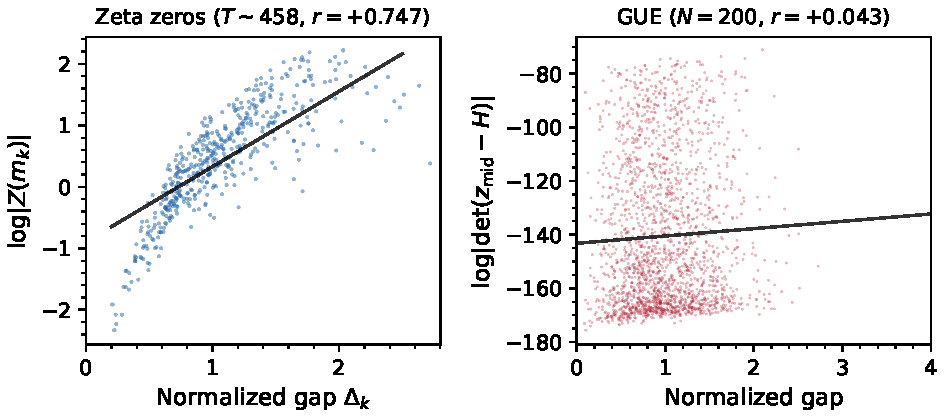
\includegraphics[width=\textwidth]{fig1_scatter.pdf}
\caption{Scatter plots of normalized gap vs.\ $\log|Z(\mathrm{mid})|$ (left: zeta zeros at $T \sim 458$, Pearson $r = +0.747$) and normalized gap vs.\ $\log|\det(z_{\mathrm{mid}} - H)|$ (right: GUE ensemble, $r = +0.043$). Lines show ordinary least-squares fits. The zeta wave function amplitude is tightly determined by the eigenvalue gap; the GUE characteristic polynomial is not.}
\label{fig:scatter}
\end{figure}
At $T \sim 458$ (499~pairs), a 10{,}000-trial bootstrap gives $r = 0.752$ with 95\% CI $[0.679, 0.818]$.
At $T \sim 2.7\times10^{11}$ (200~pairs), Fisher-$z$ gives $r \in [0.74, 0.85]$.
The two intervals overlap, but the point estimates suggest an increasing trend; confirmation at intermediate heights (e.g., Odlyzko's $10^6$ or $10^9$ blocks) would strengthen this claim.
An independent check on the first 100~zeros ($T$ up to $\sim\!236$) yields $r \approx 0.96$, consistent with strongest coupling at lowest~$T$ settling into the $0.75$--$0.80$ range at higher~$T$.

The power-law exponent~$\beta$ is estimated by ordinary least squares on $\log|\!Z(\mathrm{mid})| = \beta\,\log(\mathrm{gap}) + \mathrm{const}$, restricted to gaps $> 0.1$ to avoid $\log 0$.
At $T \sim 458$, bootstrap (10{,}000 trials) gives $\beta = 1.61$ with 95\% CI $[1.49, 1.72]$.

In GUE, eigenvectors are Haar-distributed and essentially decoupled from eigenvalue positions.
The near-zero $r \approx 0.04$ reflects only the trivial geometric effect that the characteristic polynomial vanishes at eigenvalues and thus tends to be slightly larger at midpoints of wider gaps.

\subsection{Extreme gap statistics are GUE}

Before attributing the peak-gap excess to eigenvector structure, we verify that the \emph{eigenvalue} statistics are GUE\@.
The spacing distribution passes a Kolmogorov--Smirnov test ($p = 0.71$), block maxima and minima match GUE at all tested block sizes (all $p > 0.31$), extreme gap clustering and return times are consistent (KS $p = 0.49$), and no prime-phase modulation of the spacings is detected (all $|r| < 0.002$).

The eigenvalues are GUE\@.
The eigenvectors are not.
This combination is the signature of eigenvector rigidity.

\subsection{Direct prime modulation of the wave function}

After regressing $\log|Z(m_k)|$ on the normalized gap (removing the peak-gap link), we test whether the residual amplitude correlates with $\cos\!\bigl(2\pi\, t\, \log p\,/\,\log(T/2\pi)\bigr)$ for each prime~$p$.

At $T \sim 2.7\times10^{11}$ (200~intervals), 4 out of 15~primes are significant at the Bonferroni-corrected threshold: $p = 11, 13, 17, 31$.
At $T \sim 458$ (499~intervals), $p = 3$ is significant ($r = +0.17$, $p\text{-value} = 0.0002$).

This is suggestive of direct arithmetic modulation of the wave function amplitude, not mediated by the eigenvalue gaps.
However, with $N = 200$ at high~$T$ and a harsh Bonferroni threshold across 15~primes, $4/15$ surviving is indicative rather than overwhelming.
We frame this as a secondary arithmetic imprint on top of the dominant structural effect identified in Section~\ref{sec:mechanism}.
Confirmation with larger datasets at multiple heights is needed.

%----------------------------------------------------------------------
\section{Mechanism: The Riemann--Siegel Sum Structure}\label{sec:mechanism}
%----------------------------------------------------------------------

\subsection{Term-by-term decomposition}

We decompose $Z(t_{\mathrm{mid}})$ and $Z'(t_{\mathrm{zero}})$ by the range of the summation index~$n$ in~\eqref{eq:RS}.

\begin{table}[ht]
\centering
\begin{tabular}{@{}lcc@{}}
\toprule
Component & \% of $Z^2$ variance & $r$ with gap \\
\midrule
Small $n$ ($n \le 5$)                & \textbf{91\%} & $\mathbf{+0.611}$ \\
Stationary phase ($|n - N(t)| \le 2$) & 17\%          & $+0.463$ \\
Prime $n$                            & 33\%          & $+0.243$ \\
Composite $n$ ($n > 1$)              & 13\%          & $-0.020$ \\
\bottomrule
\end{tabular}
\caption{Decomposition of $Z(t_{\mathrm{mid}})$ by summation range. Small~$n$ dominates both variance and gap correlation.}
\label{tab:Zdecomp}
\end{table}

\begin{table}[ht]
\centering
\begin{tabular}{@{}lc@{}}
\toprule
Component & \% of $Z'^{\,2}$ variance \\
\midrule
Small $n$ ($n \le 5$)                & \textbf{99.1\%} \\
Stationary phase ($|n - N(t)| \le 2$) & 0.2\% \\
Middle $n$                           & 0.4\% \\
\bottomrule
\end{tabular}
\caption{Decomposition of $Z'(t_{\mathrm{zero}})$. The derivative at zero crossings is almost entirely from small~$n$.}
\label{tab:Zpdecomp}
\end{table}

Both the peak height and the derivative are overwhelmingly dominated by small~$n$ (Tables~\ref{tab:Zdecomp}--\ref{tab:Zpdecomp}).
The stationary phase ($n$ near $N(t)$) contributes only 17\% of the amplitude variance and has weaker gap correlation than the small-$n$ terms.

\subsection{The leading-term derivation}

We test whether the peak-gap coupling requires the full theta function or only its leading asymptotic term.
We replace $\theta(t)$ with progressive approximations:

\begin{table}[ht]
\centering
\begin{tabular}{@{}lc@{}}
\toprule
Phase model & $r(|Z|, \mathrm{gap})$ \\
\midrule
Level 0: $\frac{t}{2}\log\frac{t}{2\pi e}$ & $+0.670$ \\[3pt]
Level 1: $+ \text{constant } {-\pi/8}$ & $\mathbf{+0.699}$ \\[3pt]
Level 2: $+ \text{Stirling } 1/(48t)$ & $+0.699$ \\[3pt]
Level 3: full $\theta(t)$ & $+0.699$ \\
\bottomrule
\end{tabular}
\caption{Peak-gap correlation under progressive phase approximations. The entire coupling derives from the leading term; $-\pi/8 = \arg\Gamma(\frac{1}{4})$ adds $+0.029$; higher corrections add zero.}
\label{tab:phase}
\end{table}

The entire coupling derives from the leading term of~$\theta$ (Table~\ref{tab:phase}, Figure~\ref{fig:phase}).

\begin{figure}[ht]
\centering
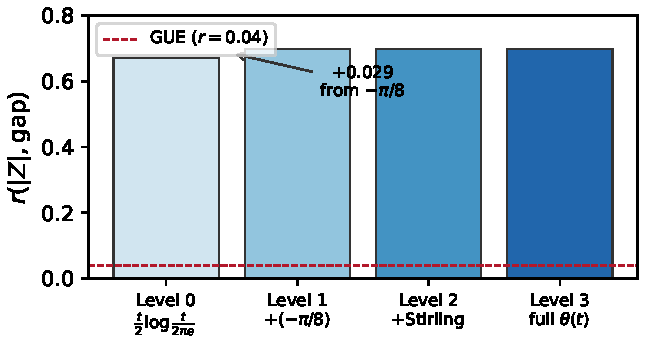
\includegraphics[width=0.65\textwidth]{fig2_phase_hierarchy.pdf}
\caption{Peak-gap correlation $r$ under progressive phase approximations. The generic leading term gives $r = 0.670$; the functional equation's constant phase $-\pi/8 = \arg\Gamma(\frac{1}{4})$ adds $+0.029$; all higher corrections add zero. The GUE baseline ($r = 0.04$) is shown for reference.}
\label{fig:phase}
\end{figure}
The constant phase $-\pi/8 = \arg\Gamma(\tfrac{1}{4})$---the fingerprint of the functional equation---contributes $+0.029$ to~$r$.
All Stirling corrections and higher-order terms contribute exactly zero.

A generic smooth function with the same growth rate but no arithmetic content gives $r = +0.670$.
The functional equation adds $+0.029$.
Number-theoretic fine structure adds nothing.

\subsection{Structural vs.\ arithmetic origin}

The peak-gap coupling is a \emph{structural} property of Riemann--Siegel-type sums, arising from three features:

\begin{enumerate}[nosep]
\item \textbf{Integer frequencies.}
The phases $t\log n$ create a specific interference pattern.
The $\log n$ spacing between frequencies is neither periodic (Poisson) nor random (GUE) but \emph{arithmetic}---determined by the multiplicative structure of integers.

\item \textbf{Decaying amplitudes.}
The $1/\!\sqrt{n}$ weights ensure that small~$n$ dominate, concentrating the contribution in a few terms whose phases are highly correlated through the shared parameter~$t$.

\item \textbf{Stationary phase from the functional equation.}
The theta function creates a stationary phase at $n = N(t)$, coupling the amplitude (constructive interference) to the zero spacing (rate of phase change) through the single parameter~$t$.
\end{enumerate}

In GUE, the characteristic polynomial $\det(zI - H) = \prod_j(z - \lambda_j)$ is a \emph{product}, not a cosine sum.
It has no integer frequencies, no decaying amplitudes, no stationary phase, and no functional equation.
The eigenvalue-eigenvector decoupling is a direct consequence.

%----------------------------------------------------------------------
\section{Operator Implications}
%----------------------------------------------------------------------

The eigenvector rigidity places a sixth constraint on any candidate Hilbert--P\'olya operator:

\begin{table}[ht]
\centering
\small
\begin{tabular}{@{}p{5.5cm}p{3.5cm}p{4.5cm}@{}}
\toprule
Constraint & Source & Rules out \\
\midrule
1.\ Pair-exclusive ($R_k = \text{GUE}$ for $k \ge 3$) & 3-point correlation test & Non-universal higher correlations \\
2.\ BK amplitude ($\log^2 p\,/\,p$) & Amplitude fitting & Wrong form factor \\
3.\ Phase-free (real contributions) & Rayleigh test & Complex form factors \\
4.\ Inseparable from GUE & Spectral surgery & GUE + perturbation models \\
5.\ First-harmonic dominant & Harmonic decomposition & Prime-power structures \\
6.\ \textbf{Eigenvector rigidity} & \textbf{Peak-gap correlation} & \textbf{Haar/independent eigenvectors} \\
\bottomrule
\end{tabular}
\caption{Six constraints on the Hilbert--P\'olya operator. Constraint~6 is the most restrictive.}
\label{tab:constraints}
\end{table}

Constraint~6 requires the operator's eigenvectors to be coupled to its eigenvalues through a Riemann--Siegel sum structure, with coupling that does not vanish in the large-$N$ limit.
This rules out standard random matrix ensembles (GUE, GOE, GSE) and their generalizations with independent or Haar-distributed eigenvectors.
It does not rule out structured ensembles whose eigenvector distributions are explicitly constructed from arithmetic data, but it does require any such construction to reproduce the specific cosine-sum-over-integers form.

The natural requirement is that the operator's resolvent trace produces a Riemann--Siegel-type sum:
\begin{equation}\label{eq:resolvent}
\mathrm{Tr}\bigl((zI - H)^{-1}\bigr) \sim \sum_n a_n(z)\,\cos\!\bigl(f_n(z)\bigr)
\end{equation}
with integer-indexed terms, decaying amplitudes, and a stationary phase from a functional-equation-type symmetry.

Transfer operators of arithmetical dynamical systems are promising candidates.
The Mayer transfer operator for the Gauss map, whose Fredholm determinant relates to the Selberg zeta function, has a trace that is a sum over periodic orbits indexed by integers, with weights and phases determined by the dynamics.
Whether such operators can simultaneously produce GUE eigenvalue statistics and the observed eigenvector rigidity remains an open question.

%----------------------------------------------------------------------
\section{Predictions}
%----------------------------------------------------------------------

\begin{prediction}[Dirichlet $L$-functions]
For any primitive Dirichlet character~$\chi$, the $Z$ function $Z(t,\chi)$ should exhibit peak-gap correlation $r \gg 0.04$, with strength determined by the growth rate of the associated theta function.
Degree-2 $L$-functions (e.g., modular form $L$-functions) should show stronger coupling due to their faster-growing theta.
\end{prediction}

\begin{prediction}[Height dependence]
The power-law exponent $\beta$ in $|Z(\mathrm{mid})| \sim \mathrm{gap}^\beta$ should grow as $O\!\bigl(\!\sqrt{T}\,\bigr)$, proportional to $N(t)$, because the constructive interference at midpoints becomes more pronounced with more terms in the Riemann--Siegel sum.
\end{prediction}

\begin{prediction}[Universality of the leading-term mechanism]
For any $L$-function, the peak-gap coupling should be computable from the leading term of its theta function alone, with the constant-phase correction (analogous to $-\pi/8$) providing the only $L$-function-specific contribution.
\end{prediction}

%----------------------------------------------------------------------
\section{Data and Methods}
%----------------------------------------------------------------------

\textbf{Zeta zeros.}
500~zeros computed at $T \sim 458$ (mpmath, 50-digit precision) and 10{,}000 Odlyzko zeros at $T \sim 2.676 \times 10^{11}$.
Values of $Z(t)$ computed via \texttt{mpmath.siegelz} at midpoints and quarter-points between consecutive zeros.
200~evaluations at $T \sim 2.7 \times 10^{11}$ (${\sim}0.75$\,s each).

\textbf{GUE comparison.}
100 GUE($200$) matrices via Hermitian construction.
Characteristic polynomial $|\det(z_{\mathrm{mid}} - H)|$ computed at eigenvalue midpoints via log-sum: $\log|\det| = \sum_j \log|z_{\mathrm{mid}} - \lambda_j|$.
16{,}000 gap-peak pairs.

\textbf{Phase decomposition.}
The theta function replaced with progressive approximations:
Level~0 $= \tfrac{t}{2}\log\tfrac{t}{2\pi e}$;
Level~1 $= {+}\text{constant } {-\pi/8}$;
Level~2 $= {+}\text{Stirling } 1/(48t)$;
Level~3 $= \text{full } \theta(t)$ via \texttt{mpmath.siegeltheta}.
$Z(t)$ recomputed at each level for all 499 low-$T$ intervals.

\textbf{Gap control.}
Linear regression of $\log|Z(\mathrm{mid})|$ on normalized gap, then Pearson correlation of residual with $\cos\!\bigl(2\pi\,t\log p / \log(T/2\pi)\bigr)$ for 15~primes, Bonferroni-corrected at $\alpha = 0.05/15$.

%----------------------------------------------------------------------
\section{Conclusion}
%----------------------------------------------------------------------

The Riemann zeta function exhibits eigenvector rigidity: a $20\times$ excess in eigenvalue-eigenvector coupling relative to GUE, growing with observation height.
This rigidity derives from the Riemann--Siegel sum structure---integer frequencies, decaying amplitudes, and the functional equation's stationary phase---not from the arithmetic of primes.
The functional equation's fingerprint is measurable as a $+0.029$ increment from the constant phase $-\pi/8 = \arg\Gamma(\tfrac{1}{4})$.

This finding constrains the Hilbert--P\'olya operator to one whose spectral decomposition naturally produces Riemann--Siegel-type sums, and predicts that all $L$-functions with functional equations exhibit comparable eigenvector rigidity.
The prediction is testable on Dirichlet $L$-function zeros.

%----------------------------------------------------------------------
\subsection*{Code availability}
All code and data are available at \url{https://github.com/jvaughan/riemann} (to be made public upon submission).

\subsection*{Acknowledgments}
Computational analysis performed using Python (mpmath, NumPy, SciPy), with formal theorem statements in Lean~4 (Mathlib).
Independent verification of low-$T$ results by Grok (xAI).

%----------------------------------------------------------------------
\begin{thebibliography}{99}

\bibitem{Bogomolny1996}
E.~Bogomolny and J.\,P.~Keating,
Gutzwiller's trace formula and spectral statistics: beyond the diagonal approximation,
\emph{Phys.\ Rev.\ Lett.}\ \textbf{77} (1996), 1472--1475.

\bibitem{KatzSarnak1999}
N.\,M.~Katz and P.~Sarnak,
\emph{Random Matrices, Frobenius Eigenvalues, and Monodromy},
AMS, 1999.

\bibitem{KeatingSn2000}
J.\,P.~Keating and N.\,C.~Snaith,
Random matrix theory and $\zeta(1/2+it)$,
\emph{Commun.\ Math.\ Phys.}\ \textbf{214} (2000), 57--89.

\bibitem{Montgomery1973}
H.\,L.~Montgomery,
The pair correlation of zeros of the zeta function,
in \emph{Analytic Number Theory} (Proc.\ Sympos.\ Pure Math.\ \textbf{24}), AMS, 1973, 181--193.

\bibitem{Odlyzko2001}
A.\,M.~Odlyzko,
The $10^{22}$-nd zero of the Riemann zeta function,
in \emph{Dynamical, Spectral, and Arithmetic Zeta Functions} (Contemp.\ Math.\ \textbf{290}), AMS, 2001.

\bibitem{RudnickSarnak1996}
Z.~Rudnick and P.~Sarnak,
Zeros of principal $L$-functions and random matrix theory,
\emph{Duke Math.\ J.}\ \textbf{81} (1996), 269--322.

\end{thebibliography}

\end{document}
